% This is samplepaper.tex, a sample chapter demonstrating the
% LLNCS macro package for Springer Computer Science proceedings;
% Version 2.21 of 2022/01/12
%
\documentclass[runningheads]{llncs}
%
\usepackage[T1]{fontenc}
\usepackage[expansion=false]{microtype}
% T1 fonts will be used to generate the final print and online PDFs,
% so please use T1 fonts in your manuscript whenever possible.
% Other font encondings may result in incorrect characters.
%
\usepackage{graphicx}
\graphicspath{ {./images/} }
% Used for displaying a sample figure. If possible, figure files should
% be included in EPS format.
%
% If you use the hyperref package, please uncomment the following two lines
% to display URLs in blue roman font according to Springer's eBook style:
%\usepackage{color}
%\renewcommand\UrlFont{\color{blue}\rmfamily}
%\urlstyle{rm}
%
\begin{document}
%
\title{Building a CNN for Rock-Paper-Scissors Classification}
%
%\titlerunning{Abbreviated paper title}
% If the paper title is too long for the running head, you can set
% an abbreviated paper title here
%
\author{Lorenzo Pacacussi}
%
\authorrunning{L. Pacacussi}
% First names are abbreviated in the running head.
% If there are more than two authors, 'et al.' is used.
%

\institute{\email{lorenzopacacussi@unimi.it}\\ State university of Milano, Milan, Italy\\}
%
\maketitle              % typeset the header of the contribution
%
\begin{abstract}
This project aims to build and compare three different convolutional neural networks (CNNs) for classifying images of hand gestures representing rock, paper, scissors. 
The three CNNs represent three increasing levels of complexity and were trained on the same starndardized dataset containing 2188 images of hand gestures.
The training was performed using a train test split of 70/% and 30/% (which was then slpit into a validation set and a test set). 
Testing was performed using both the test set from the standardized dataset and two custom datasets containing 70 and 40 images respectively, which were collected by the author and contain more challenging images (e.g. with different backgrounds, lighting conditions, hand orientations, etc.).
Results show that the most complete CNN acheved the best performance on the standardized test set, with higher validation accuracy than training accuracy, which suggests that the model is not overfitting and is able to generalize well to unseen data.
However, the performance on the custom datasets was significantly lower, especially on the second custom dataset which contains images with different backgrounds where the model's performance is similar to a random classifier.
Analyzing the results, it can be observed that the model is able to correctly classify images with simple backgrounds and good lighting conditions, but struggles with images that have more complex backgrounds or poor lighting conditions. Another critical aspect is the position of the fingers, error analisys revealed that most of the misclassifications contain finger positions that are similar to other classes.






\end{abstract}
%
%
%
\section{Dataset Exploration}
The main dataset used for this project is the Kaggle Rock-Paper-Scissors dataset \cite{ref_kaggle}, which contains 2,188 images of hand gestures representing rock, paper, and scissors. The dataset is organized into three folders, one for each class, and each folder contains images with similar orientations and lighting conditions. The images are provided in JPEG format with a resolution of 300×200 pixels.

In addition to the main dataset, two secondary custom datasets were collected by the author, containing 40 and 70 images respectively. These datasets were used to evaluate the performance of the CNNs on more challenging and diverse images. The first custom dataset includes hand gesture images captured under different lighting conditions and with varying rotations, while still maintaining a homogeneous background. The second custom dataset contains images with more heterogeneous backgrounds, different camera angles, and greater variability overall. Both custom datasets are balanced, with approximately the same number of images for each class.

All datasets contain the same three classes: rock, paper, and scissors. However, the primary training dataset is highly homogeneous, as most images share similar orientations, poses, lighting conditions, and backgrounds. This homogeneity is reflected in the high performance achieved by the model on the training data. The same limitation also affects the validation and test sets, since they are generated by splitting the same original dataset used for training. As a result, these sets may not fully represent the variability encountered in real-world scenarios, making generalization to more diverse images more challenging.


\begin{figure}
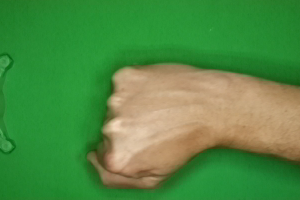
\includegraphics[width=0.3\textwidth]{rock.png}
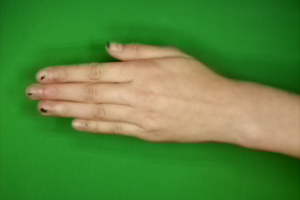
\includegraphics[width=0.3\textwidth]{paper.png}
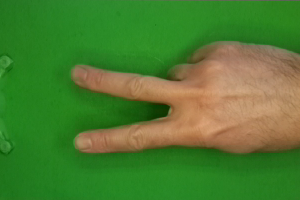
\includegraphics[width=0.3\textwidth]{scissors.png}
\caption{Sample images from the training dataset.}

\end{figure}

\section{Methodology}

\subsection{Preprocessing}
To speed up both processing and testing the images in the dataset were resized to 200x200 pixel and changed to greyscale, this allows to process only one third of the data for each image, since the color channels are reduced to one. This also means that the model will not learn any color-based feature, in this particular usecase this is a good thing since the classification is strictly shape based, color sould not influence the decisions of the model and could even be a source of overfitting, since the training dataset is very homogeneous and the images all share the same green background.
\begin{figure}
    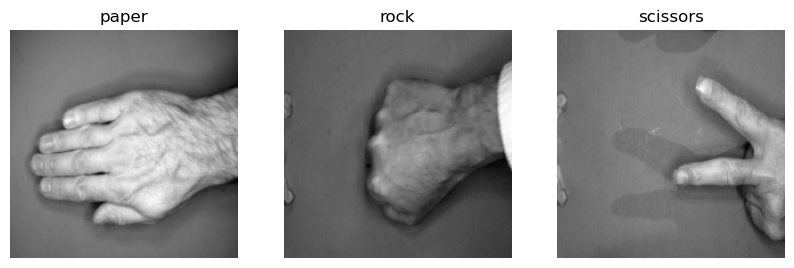
\includegraphics[width=0.9\textwidth]{rps-greyscale.png}
\end{figure}

Images were then normalized by dividing their pixel values by 255 to scale them to the range [0, 1]. This normalization step helps to improve the convergence of the CNN during training by ensuring that the input data is on a consistent scale.
This step was implemented in the code as a layer within the model, but conceptually it is a preprocessing step that is applied to the input data before it is fed into the CNN. 

The main dataset was split into a training set (70\%), a validation set (15\%), and a test set (15\%). The training set was used to train the CNNs, while the validation set was used to tune hyperparameters and prevent overfitting. The test set was reserved for evaluating the final performance of the models after training. 


\subsection{A Subsection Sample}
Please note that the first paragraph of a section or subsection is
not indented. The first paragraph that follows a table, figure,
equation etc.
does not need an indent, either.

Subsequent paragraphs, however, are indented.

\subsubsection{Sample Heading (Third Level)} Only two levels of
headings should be numbered. Lower level headings remain unnumbered;
they are formatted as run-in headings.

\paragraph{Sample Heading (Fourth Level)}
The contribution should contain no more than four levels of




\noindent Displayed equations are centered and set on a separate
line.
\begin{equation}
x + y = z
\end{equation}
Please try to avoid rasterized images for line-art diagrams and
schemas. Whenever possible, use vector graphics instead 

\begin{theorem}
This is a sample theorem. The run-in heading is set in bold, while
the following text appears in italics. Definitions, lemmas,
propositions, and corollaries are styled the same way.
\end{theorem}
%
% the environments 'definition', 'lemma', 'proposition', 'corollary',
% 'remark', and 'example' are defined in the LLNCS documentclass as well.
%
\begin{proof}
Proofs, examples, and remarks have the initial word in italics,
while the following text appears in normal font.
\end{proof}
For citations of references, we prefer the use of square brackets
and consecutive numbers. Citations using labels or the author/year
convention are also acceptable. The following bibliography provides
a sample reference list with entries for journal


\begin{credits}
\subsubsection{\ackname} A bold run-in heading in small font size at the end of the paper is
used for general acknowledgments, for example: This study was funded
by X (grant number Y).

\subsubsection{\discintname}
It is now necessary to declare any competing interests or to specifically
state that the authors have no competing interests. Please place the
statement with a bold run-in heading in small font size beneath the
(optional) acknowledgments\footnote{If EquinOCS, our proceedings submission
system, is used, then the disclaimer can be provided directly in the system.},
for example: The authors have no competing interests to declare that are
relevant to the content of this article. Or: Author A has received research
grants from Company W. Author B has received a speaker honorarium from
Company X and owns stock in Company Y. Author C is a member of committee Z.
\end{credits}
%
% ---- Bibliography ----
%
% BibTeX users should specify bibliography style 'splncs04'.
% References will then be sorted and formatted in the correct style.
%
% \bibliographystyle{splncs04}
% \bibliography{mybibliography}
%
\begin{thebibliography}{8}
\bibitem{ref_article1}
Author, F.: Article title. Journal \textbf{2}(5), 99--110 (2016)

\bibitem{ref_lncs1}
Author, F., Author, S.: Title of a proceedings paper. In: Editor,
F., Editor, S. (eds.) CONFERENCE 2016, LNCS, vol. 9999, pp. 1--13.
Springer, Heidelberg (2016). \doi{10.10007/1234567890}

\bibitem{ref_book1}
Author, F., Author, S., Author, T.: Book title. 2nd edn. Publisher,
Location (1999)

\bibitem{ref_proc1}
Author, A.-B.: Contribution title. In: 9th International Proceedings
on Proceedings, pp. 1--2. Publisher, Location (2010)

\bibitem{ref_url1}
LNCS Homepage, \url{http://www.springer.com/lncs}, last accessed 2023/10/25

\bibitem{ref_kaggle}
Author, Julien de la Bruère-Terreault: Rock Paper Scissors Dataset. Kaggle, https://www.kaggle.com/datasets/drgfreeman/rockpaperscissors/data (2023)
\end{thebibliography}
\end{document}
